\documentclass[12pt,a4paper]{report}

% ------------------------------------------------
% Packages
% ------------------------------------------------

\usepackage[a4paper,
            left=1in,
            right=1in,
            top=1in,
            bottom=1in]{geometry}

\usepackage{graphicx}
\usepackage{fancyhdr}
\usepackage{titlesec}
\usepackage{hyperref}
\usepackage{amsmath,amssymb}
\usepackage{float}
\usepackage{caption}
\usepackage{booktabs}
\usepackage{array}
\usepackage{longtable}
\usepackage{tabularx}
\usepackage{adjustbox}

% ------------------------------------------------
% Formatting
% ------------------------------------------------

\linespread{1.3}

\titleformat{\chapter}[display]
{\normalfont\bfseries}
{}{0pt}
{\centering\Huge}

\titleformat{\section}
{\large\bfseries}
{\thesection}
{1em}
{}

\titleformat{\subsection}
{\normalsize\bfseries}
{\thesubsection}
{1em}
{}

\titleformat{\subsubsection}
{\small\bfseries}
{\thesubsubsection}
{1em}
{}

\titlespacing*{\chapter}{0pt}{-20pt}{20pt}

% ------------------------------------------------
% Hyperlinks
% ------------------------------------------------

\hypersetup{
    colorlinks=true,
    linkcolor=black,
    urlcolor=blue,
    citecolor=black
}

% ------------------------------------------------
% Header / Footer
% ------------------------------------------------

\pagestyle{fancy}
\fancyhf{}

\fancyfoot[C]{\thepage}

\renewcommand{\headrulewidth}{0pt}
\renewcommand{\footrulewidth}{0pt}

% ------------------------------------------------
% Document
% ------------------------------------------------

\begin{document}

% =================================================
% TITLE PAGE
% =================================================

\begin{titlepage}

\centering

\textbf{\Large GOVERNMENT OF KERALA}

\vspace{0.4cm}

\textbf{\Large DEPARTMENT OF TECHNICAL EDUCATION}

\vspace{0.8cm}

\textbf{\Large RAJIV GANDHI INSTITUTE OF TECHNOLOGY}

\vspace{0.4cm}

\textbf{\Large (GOVT. ENGINEERING COLLEGE)}

\vspace{0.4cm}

\textbf{\Large KOTTAYAM - 686501}

\vspace{1.5cm}


\includegraphics[width=0.25\textwidth]{image.png}

\vspace{1.5cm}

{\Large\textbf{MINI PROJECT REPORT}}

\vspace{0.8cm}

{\LARGE\textbf{SENTIO}}

\vspace{0.4cm}

{\large
An AI-Powered Real-Time Interactive Presentation and Audience Engagement Platform
}

\vfill

\textbf{SONET SHAJI}

\vspace{0.3cm}

Master of Computer Applications

\vspace{0.3cm}

Reg. No. 25MP2457

\vspace{0.8cm}

2026

\end{titlepage}

% =================================================
% FRONT MATTER
% =================================================

\pagenumbering{roman}
\newpage
\thispagestyle{empty}

\begin{center}
{\Large\textbf{ABSTRACT}}
\end{center}

\vspace{1cm}

Presentations have long been the standard way to share knowledge in classrooms, seminars, and business meetings. However, most presentations remain a one-way street where the speaker talks and the audience simply listens. When speakers try to make sessions interactive using separate polling apps or quiz tools, they often run into frustrating workflow issues—having to switch browser tabs constantly, juggle multiple links, or ask the audience to enter different room codes. This friction breaks the natural flow of the presentation.

To solve these practical problems, this project introduces \textbf{Sentio}, an interactive presentation platform that brings slide design, live audience participation, and artificial intelligence together into a single web application. Sentio is built around a fixed 16:9 canvas layout, meaning text, images, and interactive questions stay exactly where they are placed without shifting or overflowing on different screens. Presenters can add live multiple-choice polls, timed quizzes, rating scales, word clouds, and open Q\&A directly onto their slides.

The system is developed using modern web technologies. The frontend uses \textbf{Next.js 15} and \textbf{React 19} with \textbf{Tailwind CSS} for a clean and responsive interface. Real-time updates are handled seamlessly using \textbf{Socket.IO} on a \textbf{Node.js} and \textbf{Express.js} backend, so audience votes and quiz answers appear instantly on the presenter's screen. The platform also integrates \textbf{Groq AI} (powered by LLaMA 3.3) to help presenters quickly generate structured slides, create quiz questions, and summarize session feedback. All data is securely stored in \textbf{MongoDB}, and automated PDF summary reports can be downloaded after each session.

By combining an intuitive slide editor with instant live responses and AI assistance, Sentio helps presenters deliver engaging, interactive, and memorable presentations with minimal preparation effort.

\vfill

\noindent
\textbf{Keywords:} Interactive Presentations, Audience Engagement, Real-Time WebSockets, Next.js, React, Node.js, Groq AI, MongoDB, Canvas Layout.
\tableofcontents

\clearpage

\listoffigures

\clearpage

\listoftables

\clearpage

% =================================================
% MAIN REPORT
% =================================================

\pagenumbering{arabic}

\setcounter{page}{1}

\chapter{Introduction}

\section{Background}

Presentations are an essential part of how we communicate ideas in colleges, universities, corporate offices, and technical conferences. For decades, computerized presentation tools like Microsoft PowerPoint and Google Slides have served as the standard way to prepare visual aids. While these tools make it easy to format text, add graphics, and show bullet points, they are fundamentally designed for one-way broadcasting. The presenter speaks, the slides advance, and the audience remains passive spectators.

In modern educational and professional settings, passive listening often results in short attention spans and low retention rates. Educational research has repeatedly shown that active learning—where listeners participate through questions, polls, and discussions—greatly improves understanding and keeps participants focused.

To make sessions more engaging, many speakers try using third-party polling tools such as Mentimeter, Slido, or Kahoot. However, because these tools are separate from standard presentation software, presenters must constantly switch between their presentation slides and a web browser window during live talks. Audience members must also visit separate websites, enter room codes, and wait for popups. This constant back-and-forth disrupts the speaker's rhythm and distracts the audience.

\textbf{Sentio} was created to eliminate this friction. Sentio is a unified, web-based presentation platform that integrates visual slide authoring, live audience polling, competitive quizzes, and AI assistance into a single, cohesive tool.

\section{Problem Statement}

Presenters and audiences regularly face several practical difficulties during live presentations:

\begin{enumerate}
    \item \textbf{Passive and Disengaged Audiences:} Traditional slide tools provide no built-in way for listeners to participate, ask questions, or share feedback during a talk.
    \item \textbf{Tool Switching and Presentation Friction:} Juggling separate applications for slides, live polls, and Q\&A creates awkward pauses, screen flickering, and technical confusion during presentations.
    \item \textbf{Rigid Question Layouts:} Most polling tools display questions as fixed full-screen takeovers, preventing presenters from combining questions with explanatory text, code snippets, or diagrams on the same slide.
    \item \textbf{High Preparation Overhead:} Manually brainstorming and drafting interactive quiz questions, distractors, and discussion topics takes considerable time and effort.
\end{enumerate}

Sentio directly addresses these challenges by offering an all-in-one presentation environment where interactive elements sit directly on the slide canvas, synchronized in real time via WebSockets and supported by fast generative AI.

\section{Objectives}

The core objectives of the Sentio project are:

\begin{itemize}
    \item \textbf{Develop a 16:9 Canvas Slide Editor:} Build a flexible visual editor that maintains a reliable 16:9 aspect ratio across all screen sizes without shifting elements or clipping content.
    \item \textbf{Integrate Live Interaction Elements:} Allow presenters to place live quizzes, multiple-choice polls, rating matrices, word clouds, Q\&A boards, and leaderboards directly on any slide.
    \item \textbf{Provide Sub-Second Real-Time Synchronization:} Implement a high-speed WebSocket engine using Socket.IO so audience responses, timer updates, and slide transitions happen with near-zero latency.
    \item \textbf{Embed Fast AI Slide Generation:} Integrate Groq AI with the LLaMA 3.3 model to automatically create complete slide decks, quiz questions, and summaries from simple topic prompts or uploaded documents.
    \item \textbf{Deliver Role-Specific Views:} Create tailored interfaces for Presenters (with private speaker notes and live controls), Projectors (a clean display without clutter), and Participants (a touch-friendly mobile interface).
    \item \textbf{Automate Post-Session Analytics:} Provide detailed session attendance, response breakdowns, and downloadable PDF reports.
\end{itemize}

\section{Scope}

The scope of the Sentio platform covers:

\begin{itemize}
    \item \textbf{Slide Studio:} An intuitive 3-panel builder with slide thumbnail navigation, a visual drag-and-drop canvas, and a context-sensitive properties panel with automatic saving.
    \item \textbf{Audience Participation:} A lightweight mobile web client that allows audience members to join instantly using a 6-character PIN or QR code without requiring an account.
    \item \textbf{Live Host Controls:} Presenter tools for starting timers, locking responses, revealing correct answers, and displaying real-time leaderboards.
    \item \textbf{User and Organization Management:} Secure account registration, JWT authentication, password encryption, and multi-user organization workspaces.
    \item \textbf{Reporting:} Instant generation of clean, downloadable PDF summary reports at the conclusion of every presentation.
\end{itemize}

\section{Relevance}

Sentio brings clear value to modern presentations:

\begin{itemize}
    \item \textbf{For Educators and Trainers:} Helps instructors gauge student understanding on the spot and immediately address topics where students struggle.
    \item \textbf{For Speakers and Presenters:} Eliminates the need to buy and manage multiple software subscriptions by unifying slides and polling in one application.
    \item \textbf{From a Software Engineering Standpoint:} Combines modern full-stack web technologies—including Next.js 15, React 19, TypeScript, Socket.IO, and Groq AI—into a maintainable monorepo architecture.
\end{itemize}

\section{Report Organization}

The report is structured into the following chapters:

\begin{itemize}
    \item \textbf{Chapter 2 (System Study):} Examines existing systems, analyzes their limitations, introduces the proposed platform, and details the feasibility study.
    \item \textbf{Chapter 3 (Development Methodology):} Explains the Agile Scrum methodology, sprint planning, and the justification for the chosen technology stack.
    \item \textbf{Chapter 4 (System Design):} Presents the architectural blueprints, data flow diagrams, UML diagrams, and database schemas.
    \item \textbf{Chapter 5 (Implementation and Results):} Covers the development of the frontend and backend modules, testing procedures, and system results.
    \item \textbf{Chapter 6 (Conclusion and Future Scope):} Summarizes the project achievements, notes current limitations, and outlines future enhancements.
\end{itemize}

\chapter{System Study}

\section{Introduction}

Before building Sentio, an in-depth study was conducted to understand how presenters currently deliver talks, where existing tools fall short, and what technical requirements are necessary to build a truly integrated interactive presentation platform. This chapter reviews existing market solutions, outlines their limitations, introduces the proposed Sentio platform, and presents the project's feasibility analysis.

\section{Existing Systems and Market Analysis}

Currently, speakers and educators rely on two main categories of software:

\begin{enumerate}
    \item \textbf{Traditional Presentation Software:} Tools such as Microsoft PowerPoint, Google Slides, and Apple Keynote. These applications are great for designing visually appealing slide decks with custom fonts, images, and animations. However, they were built solely for one-way broadcasting. They offer no built-in way to collect live audience feedback, run quizzes, or track comprehension while presenting.
    
    \item \textbf{Standalone Audience Response Platforms:} Web applications such as Mentimeter, Slido, and Kahoot. While these tools allow audience members to vote and submit questions using their smartphones, they function as standalone web pages. Each question takes over the whole screen, making it impossible to combine questions with explanatory notes or diagrams. Furthermore, presenters have to switch back and forth between their slide deck and the polling tool during presentations, breaking the natural rhythm of the session.
\end{enumerate}

\subsection{Comparison of Systems}

Table~\ref{tab:comparison} highlights the key differences between traditional presentation tools, standalone audience polling tools, and the proposed Sentio platform.

\begin{table}[H]
\centering
\caption{Comparison of Presentation and Polling Systems}
\label{tab:comparison}
\begin{adjustbox}{max width=\textwidth}
\begin{tabular}{lcccc}
\toprule
\textbf{Feature} & \textbf{PowerPoint / Slides} & \textbf{Mentimeter} & \textbf{Kahoot} & \textbf{Sentio (Proposed)} \\
\midrule
Visual 16:9 Slide Canvas & Yes & Limited & No & \textbf{Yes} \\
Draggable Elements on Slides & Yes & No & No & \textbf{Yes} \\
Live Audience Polling & No & Yes & Yes & \textbf{Yes} \\
Real-Time WebSocket Sync & No & Yes & Yes & \textbf{Yes} \\
Built-in AI Slide Generation & Limited & Basic & Basic & \textbf{Yes (Groq LLaMA 3.3)} \\
Multiple Interactions per Slide & No & No & No & \textbf{Yes} \\
Zero-Install Mobile Joining & N/A & Yes & App / Web & \textbf{Yes (QR / PIN)} \\
Automated PDF Reports & Basic & Paid & Limited & \textbf{Yes} \\
\bottomrule
\end{tabular}
\end{adjustbox}
\end{table}

\section{Limitations of the Existing Systems}

The most significant shortcomings identified in current solutions include:

\begin{itemize}
    \item \textbf{Fragmented Workflow:} Presenters are forced to jump between slide apps and polling websites, causing awkward delays and confusing the audience.
    \item \textbf{Rigid Layouts:} Questions cannot be placed flexibly on a slide with supporting images or notes; they always take over the whole screen.
    \item \textbf{Manual Creation Effort:} Writing quizzes, answer choices, and discussion prompts from scratch takes considerable time and effort.
    \item \textbf{Multiple Subscriptions:} Schools and organizations often end up paying for separate subscriptions for slide tools and polling tools.
\end{itemize}

\section{Proposed System Overview}

\textbf{Sentio} combines slide design, audience engagement, and generative artificial intelligence into a single, cohesive web platform. 

The core features of the platform include:
\begin{itemize}
    \item A visual 16:9 canvas where text, images, and interactive questions live together naturally.
    \item A full suite of interactive tools: multiple-choice polls, live quizzes with timers, rating scales, word clouds, Q\&A boards, and leaderboards.
    \item Instant real-time updates via WebSockets so audience votes appear immediately on the main presentation display.
    \item AI-assisted slide creation powered by Groq and LLaMA 3.3 for generating complete decks and quizzes in seconds.
    \item Automatic PDF session reports summarizing attendance, participation, and quiz results.
\end{itemize}

\section{Feasibility Study}

A feasibility study was carried out to ensure the project could be built effectively within our resources:

\subsection{Technical Feasibility}
The project uses dependable, modern technologies. Next.js 15 and React 19 provide a fast and reactive frontend. Node.js, Express.js, and Socket.IO provide a dependable backend for handling high-concurrency real-time WebSocket communication. MongoDB provides flexible document storage for slide content, and Groq provides fast AI inference for slide generation. These tools are open-source and well-documented, confirming technical feasibility.

\subsection{Operational Feasibility}
Sentio is designed to be straightforward for both presenters and audience members. Presenters can create and run presentations entirely inside standard web browsers with no software installation. Audience members join instantly by scanning a QR code or entering a 6-character code on their mobile devices without needing to create an account. This zero-install approach ensures high adoption and usability.

\subsection{Economic Feasibility}
The system is built entirely with open-source frameworks and deployed on free-tier cloud hosting (Vercel and Render). This eliminates software licensing costs while providing a unified tool that removes the need for multiple paid subscriptions.

\section{System Requirements}

\subsection{Functional Requirements}
\begin{enumerate}
    \item \textbf{Account Management:} User registration, secure login, password encryption, and profile settings.
    \item \textbf{Slide Management:} Creating, editing, duplicating, reordering, and deleting presentations and slides.
    \item \textbf{Interactive Elements:} Placing and configuring Quizzes, Polls, Word Clouds, Ratings, and Q\&A panels on any slide.
    \item \textbf{Live Hosting:} Generating session PINs, broadcasting slide changes, locking responses, and revealing correct answers.
    \item \textbf{AI Slide Generation:} Generating full slide decks and quiz questions from user topic prompts or documents.
    \item \textbf{Reporting:} Generating downloadable PDF session summaries and leaderboard rankings.
\end{enumerate}

\subsection{Non-Functional Requirements}
\begin{enumerate}
    \item \textbf{Performance:} Live responses and slide transitions must update across all devices in under 100 milliseconds.
    \item \textbf{Visual Consistency:} Slide layouts must maintain a clean 16:9 aspect ratio across all display sizes.
    \item \textbf{Security:} Secure password hashing using bcrypt and protected API endpoints using JWT authentication tokens.
    \item \textbf{Usability:} Intuitive desktop controls for presenters and a simple, touch-optimized interface for mobile participants.
\end{enumerate}

\subsection{Hardware and Software Requirements}

\subsubsection{Development Environment}
\begin{itemize}
    \item \textbf{RAM:} 8 GB or higher.
    \item \textbf{Operating System:} macOS, Linux, or Windows 11.
    \item \textbf{Runtime:} Node.js v20 or higher.
    \item \textbf{Database:} MongoDB v7.x or MongoDB Atlas.
\end{itemize}

\subsubsection{User Environment}
\begin{itemize}
    \item \textbf{Presenter:} Any desktop or laptop computer with a modern web browser.
    \item \textbf{Participant:} Any smartphone, tablet, or PC with a web browser and internet connection.
\end{itemize}
\chapter{Development Methodology}

\section{Introduction}

The development methodology defines the software engineering principles, lifecycle framework, and tooling used to build the Sentio platform. Because Sentio combines real-time WebSockets, visual slide authoring, and generative artificial intelligence, an iterative \textbf{Agile Scrum} methodology was chosen to support continuous prototyping, testing, and improvement.

\section{Agile Scrum Framework}

Rather than trying to build the entire system in one massive, sequential phase, the Agile approach breaks the project into short, manageable development cycles called sprints. This iterative process allowed us to build working features quickly, test them immediately, and refine the architecture as technical challenges arose.

The project was organized into six two-week sprints. Each sprint followed a clear cycle of backlog prioritization, sprint planning, feature implementation, and automated testing.

\begin{figure}[H]
    \centering
    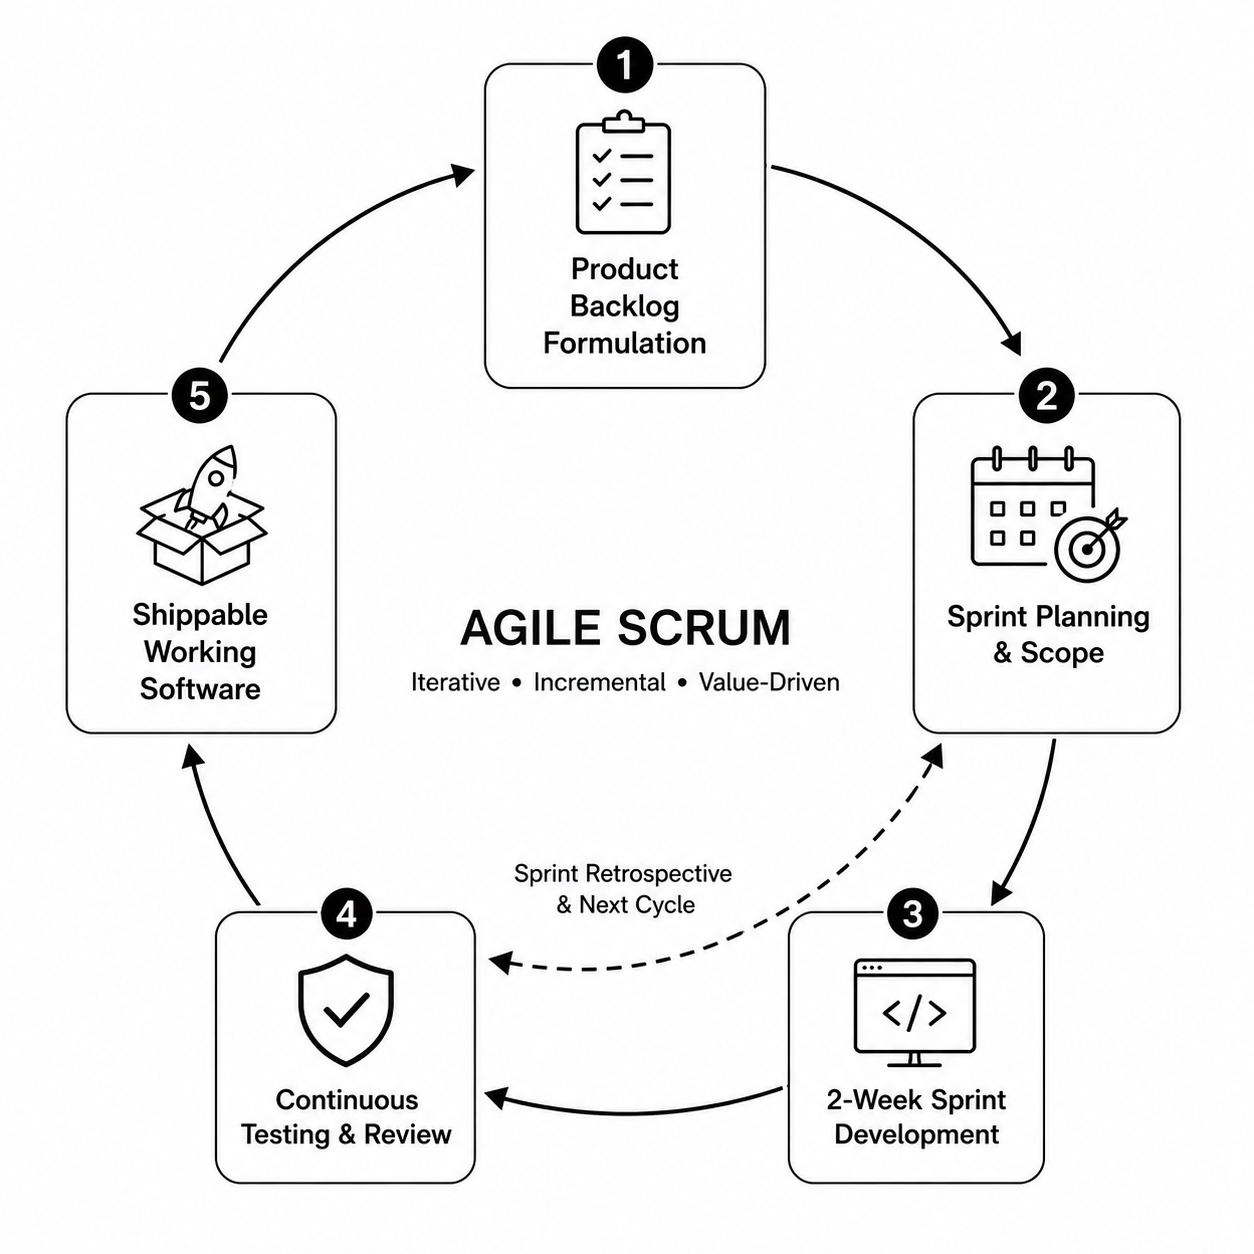
\includegraphics[width=0.85\textwidth]{figures/AgileCycle.png}
    \caption{Agile Scrum Development Cycle for Sentio}
    \label{fig:scrumcycle}
\end{figure}

\subsection{Sprint Milestones}

The core functionality of Sentio was built across distinct sprint milestones:

\begin{itemize}
    \item \textbf{Sprint 1 (Core Foundation):} Setting up the monorepo workspace, defining shared TypeScript contracts, implementing user registration, secure JWT login, and connecting to MongoDB.
    \item \textbf{Sprint 2 (Presentation Studio):} Building the user dashboard, slide management system, and the 16:9 visual canvas editor with automatic debounced saving.
    \item \textbf{Sprint 3 (Real-Time Engine):} Implementing the Socket.IO server, room-based broadcasting, presenter live controls, and the participant mobile joining screen.
    \item \textbf{Sprint 4 (Interactive Elements):} Developing the full suite of interactive components—quizzes with timers, live polls, word clouds, star ratings, and the competitive leaderboard.
    \item \textbf{Sprint 5 (AI Integration \& Reports):} Integrating Groq AI with the LLaMA 3.3 model for instant slide generation and adding downloadable PDF session reports.
    \item \textbf{Sprint 6 (Testing \& Hardening):} Writing unit tests with Jest, testing API security, checking mobile responsiveness, and finalizing documentation.
\end{itemize}

\section{Monorepo Architecture}

Sentio is organized as a monorepo using npm workspaces. This architecture keeps the frontend, backend, and shared data models cleanly organized in one repository while ensuring full type safety across the entire application:

\begin{verbatim}
Sentio/
├── apps/
│   ├── frontend/         # Next.js 15 App (React 19 + Tailwind CSS)
│   └── backend/          # Node.js + Express + Socket.IO API
├── packages/
│   └── shared/           # Shared TypeScript interfaces & socket events
└── docs/                 # Project documentation
\end{verbatim}

The \texttt{shared} package acts as a single source of truth. Both the frontend and backend import data structures and socket event names directly from this package, preventing mismatch bugs during development.

\section{Technology Stack Justification}

Table~\ref{tab:techstack} provides an overview of the core technologies chosen for Sentio and the practical reasons for their selection.

\begin{table}[H]
\centering
\caption{Technology Stack Summary}
\label{tab:techstack}
\begin{adjustbox}{max width=\textwidth}
\begin{tabular}{lll}
\toprule
\textbf{Layer} & \textbf{Technology} & \textbf{Reason for Selection} \\
\midrule
Frontend & Next.js 15 \& React 19 & Fast performance, modern App Router, and clean UI components \\
Styling & Tailwind CSS & Utility-based CSS for rapid, responsive interface styling \\
Backend & Node.js \& Express.js & Asynchronous, event-driven runtime ideal for web APIs \\
Real-Time & Socket.IO v4 & Fast bidirectional communication for live audience responses \\
Database & MongoDB \& Mongoose & Flexible document storage well-suited for slide data \\
AI Engine & Groq (LLaMA 3.3) & High-speed AI inference for fast slide and quiz creation \\
PDF Reports & PDFKit & Server-side PDF creation for downloadable session summaries \\
Security & JWT \& Bcrypt & Standard secure user authentication and password hashing \\
\bottomrule
\end{tabular}
\end{adjustbox}
\end{table}

\chapter{System Design}

\section{Introduction}

The system design phase translates the project requirements into an organized technical blueprint. This chapter outlines the overall system architecture, the 16:9 canvas layout model, Data Flow Diagrams (DFDs), UML diagrams, and the database collection schemas.

\section{System Architecture}

Sentio is built using a clean 3-tier web architecture:
\begin{enumerate}
    \item \textbf{Client Presentation Layer:} Provides specialized web interfaces for Presenters (slide builder and host controls), Projectors (clean 16:9 auditorium display), and Participants (touch-friendly mobile app for voting and answering).
    \item \textbf{Application and Real-Time Gateway Layer:} An Express.js REST API handling user accounts, slide management, and AI requests, combined with a Socket.IO WebSocket server that manages live presentation rooms and instantaneous message broadcasting.
    \item \textbf{Persistence and Services Layer:} A MongoDB database for storing user profiles and presentation decks, along with Groq Cloud AI for fast slide generation and PDFKit for generating session reports.
\end{enumerate}

Figure~\ref{fig:sysarch} illustrates the system architecture and communication paths.

\begin{figure}[H]
    \centering
    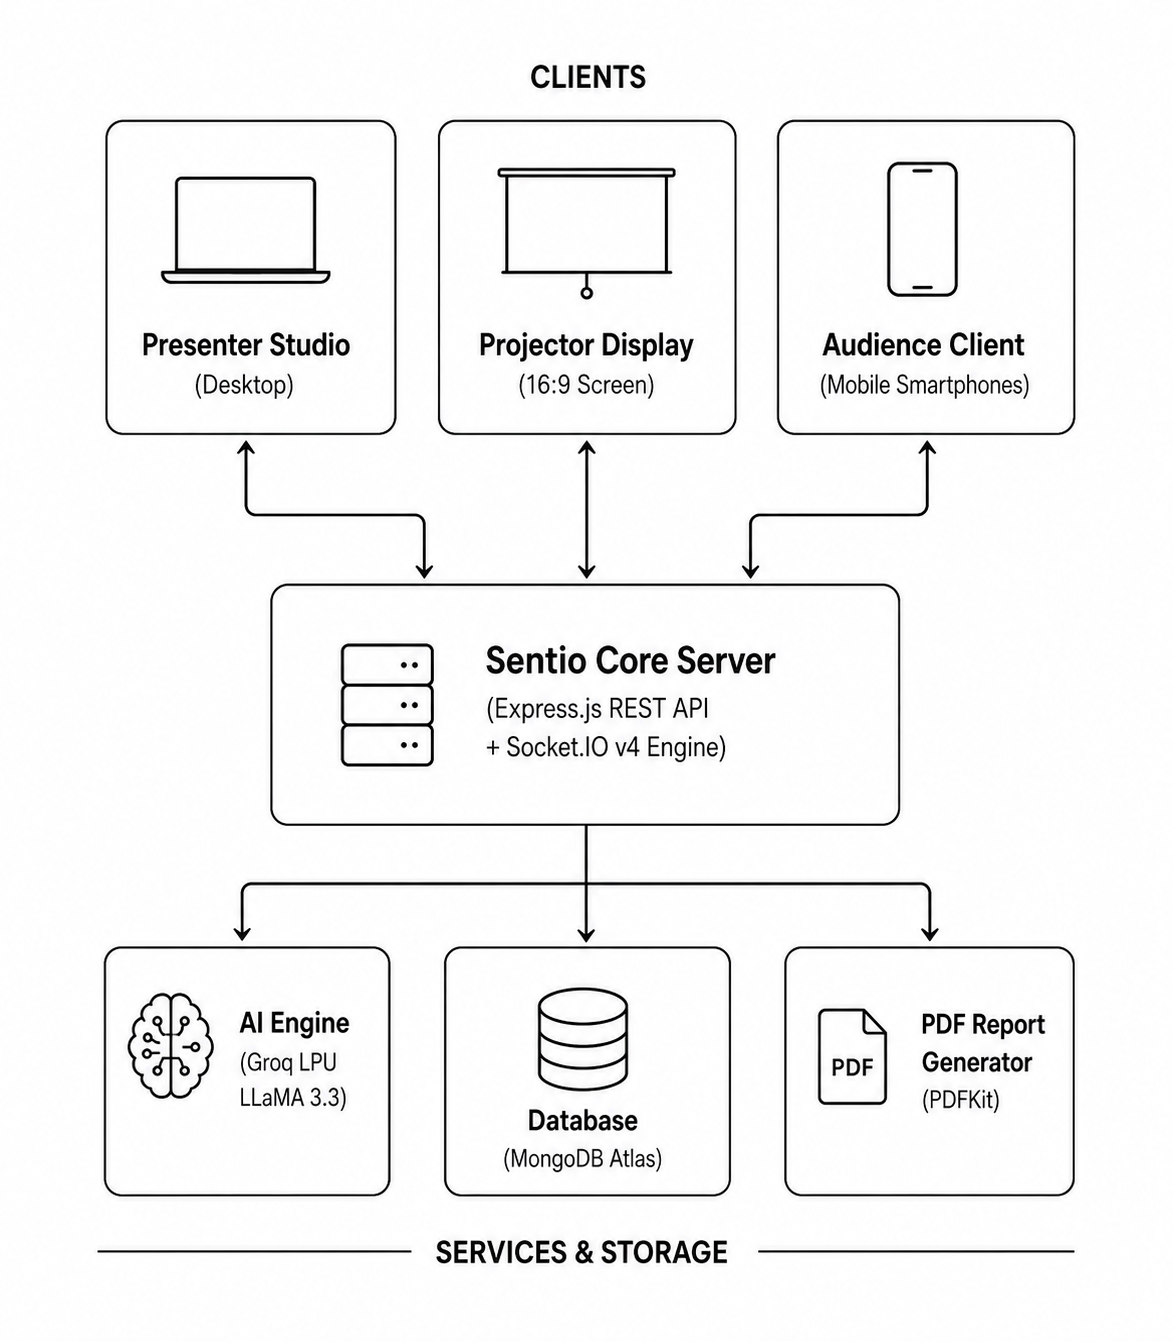
\includegraphics[width=0.9\textwidth]{figures/SentioArchitecture.png}
    \caption{System Architecture of the Sentio Platform}
    \label{fig:sysarch}
\end{figure}

\section{Slide Canvas and Coordinate System}

A fundamental feature of Sentio is the \textbf{Fixed 16:9 Slide Canvas}. In standard web development, text and buttons automatically shift and wrap when the browser window changes size. While this responsive behavior is great for regular websites, it creates problems for presentation slides where titles, images, and questions need to stay in exact visual alignment.

Sentio solves this by using a fixed 16:9 internal coordinate grid ($1920 \times 1080$ units):
\begin{itemize}
    \item Every element placed on a slide—such as headings, body text, pictures, or quiz boxes—has a fixed position and size relative to the slide canvas.
    \item The frontend measures the available screen space and automatically scales the whole slide up or down using CSS transforms while preserving the 16:9 aspect ratio.
    \item This ensures that the slide looks identical whether viewed in the editor, on a laptop, on a large auditorium projector, or on a tablet.
\end{itemize}

\begin{figure}[H]
    \centering
    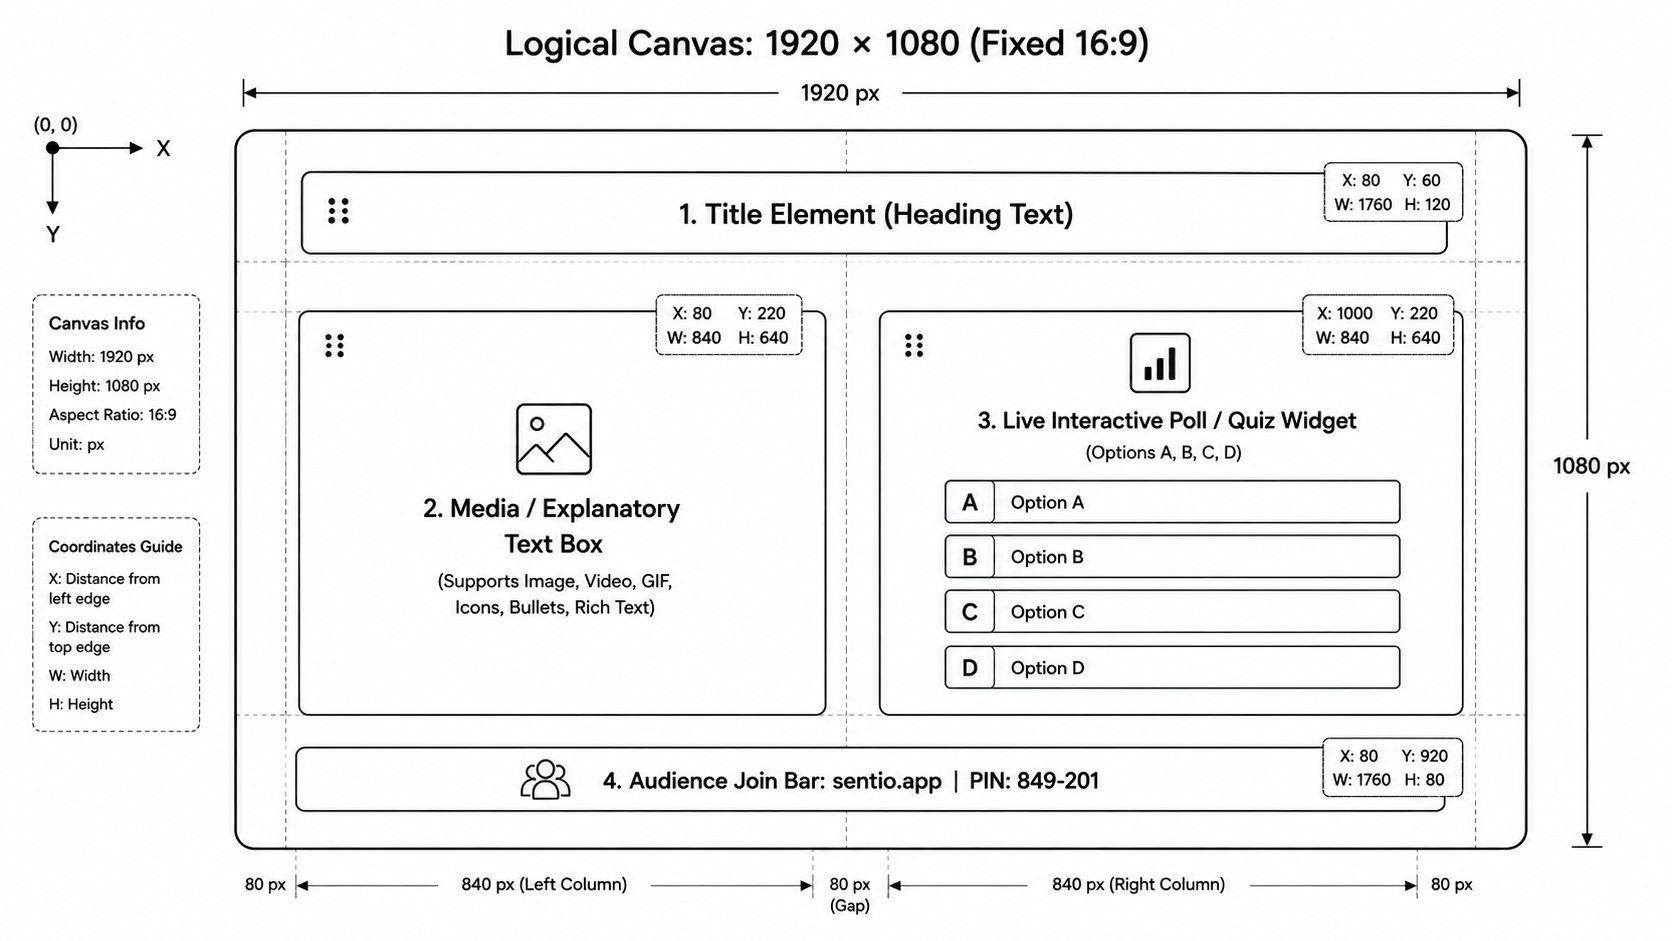
\includegraphics[width=0.85\textwidth]{figures/VisualCanvas.png}
    \caption{Visual Canvas Layout Model}
    \label{fig:canvaslayout}
\end{figure}

\section{Data Flow Diagrams}

\subsection{DFD Level 0 (Context Diagram)}
Figure~\ref{fig:dfd0} shows the high-level data flow between the external actors (Presenter, Participant, and Administrator) and the central Sentio platform.

\begin{figure}[H]
    \centering
    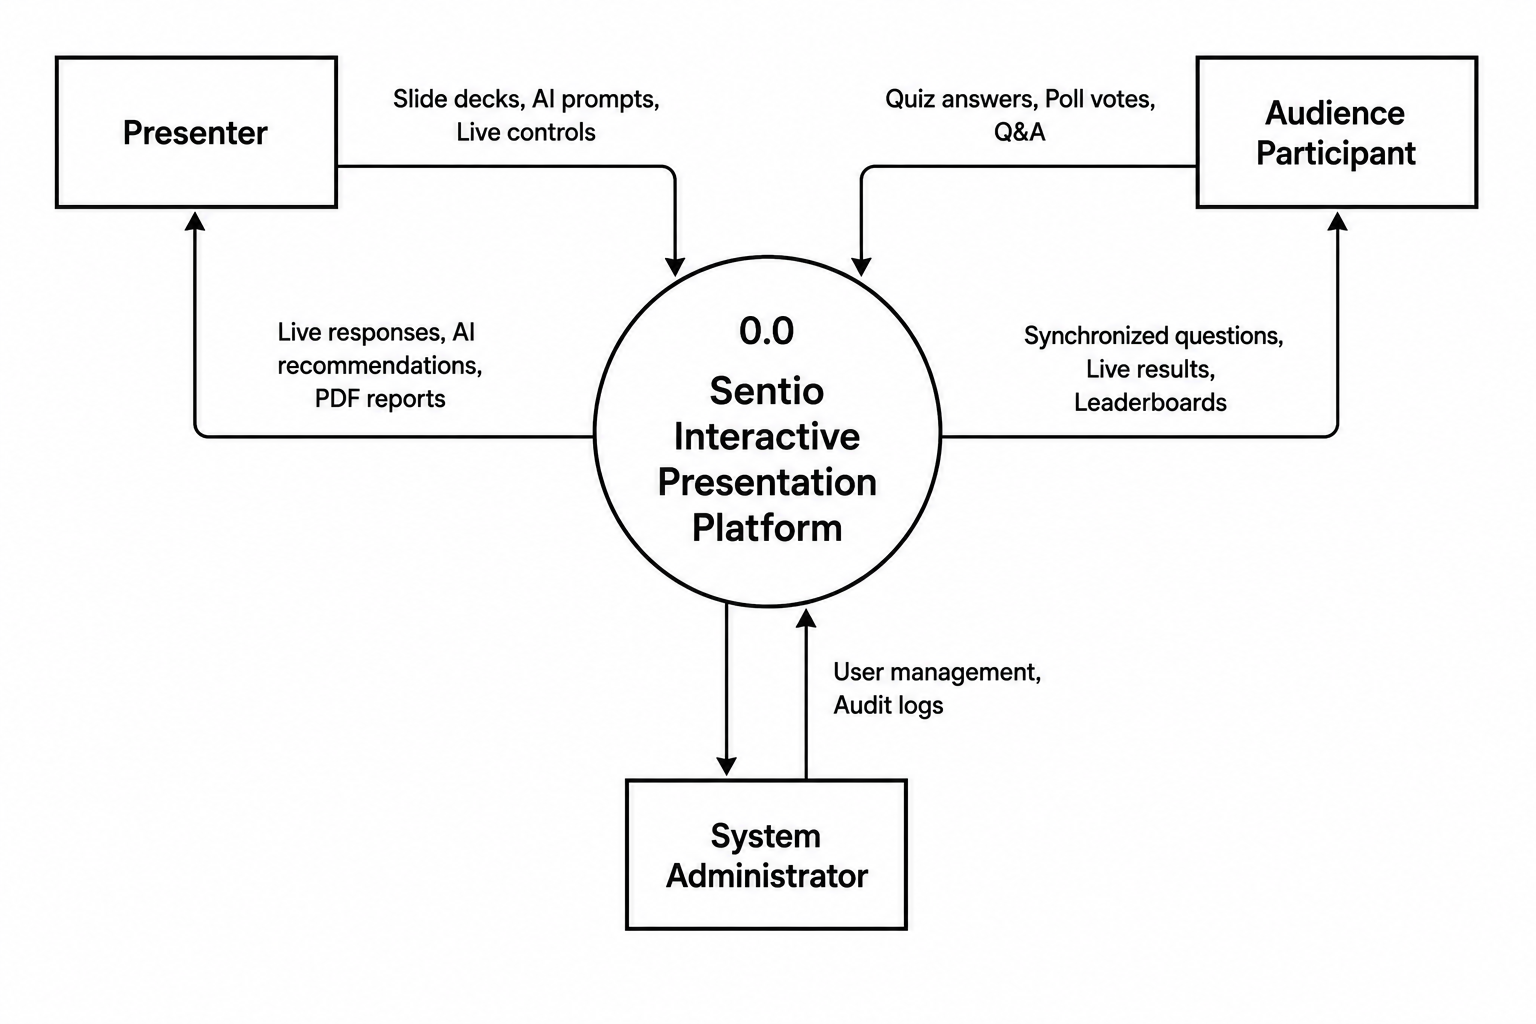
\includegraphics[width=0.85\textwidth]{figures/DFD_Level_0.png}
    \caption{Data Flow Diagram: Level 0 (Context Diagram)}
    \label{fig:dfd0}
\end{figure}

\subsection{DFD Level 1}
Figure~\ref{fig:dfd1} illustrates the internal process breakdown inside the platform, showing how authentication, slide management, AI generation, live session syncing, and reporting interact with the database.

\begin{figure}[H]
    \centering
    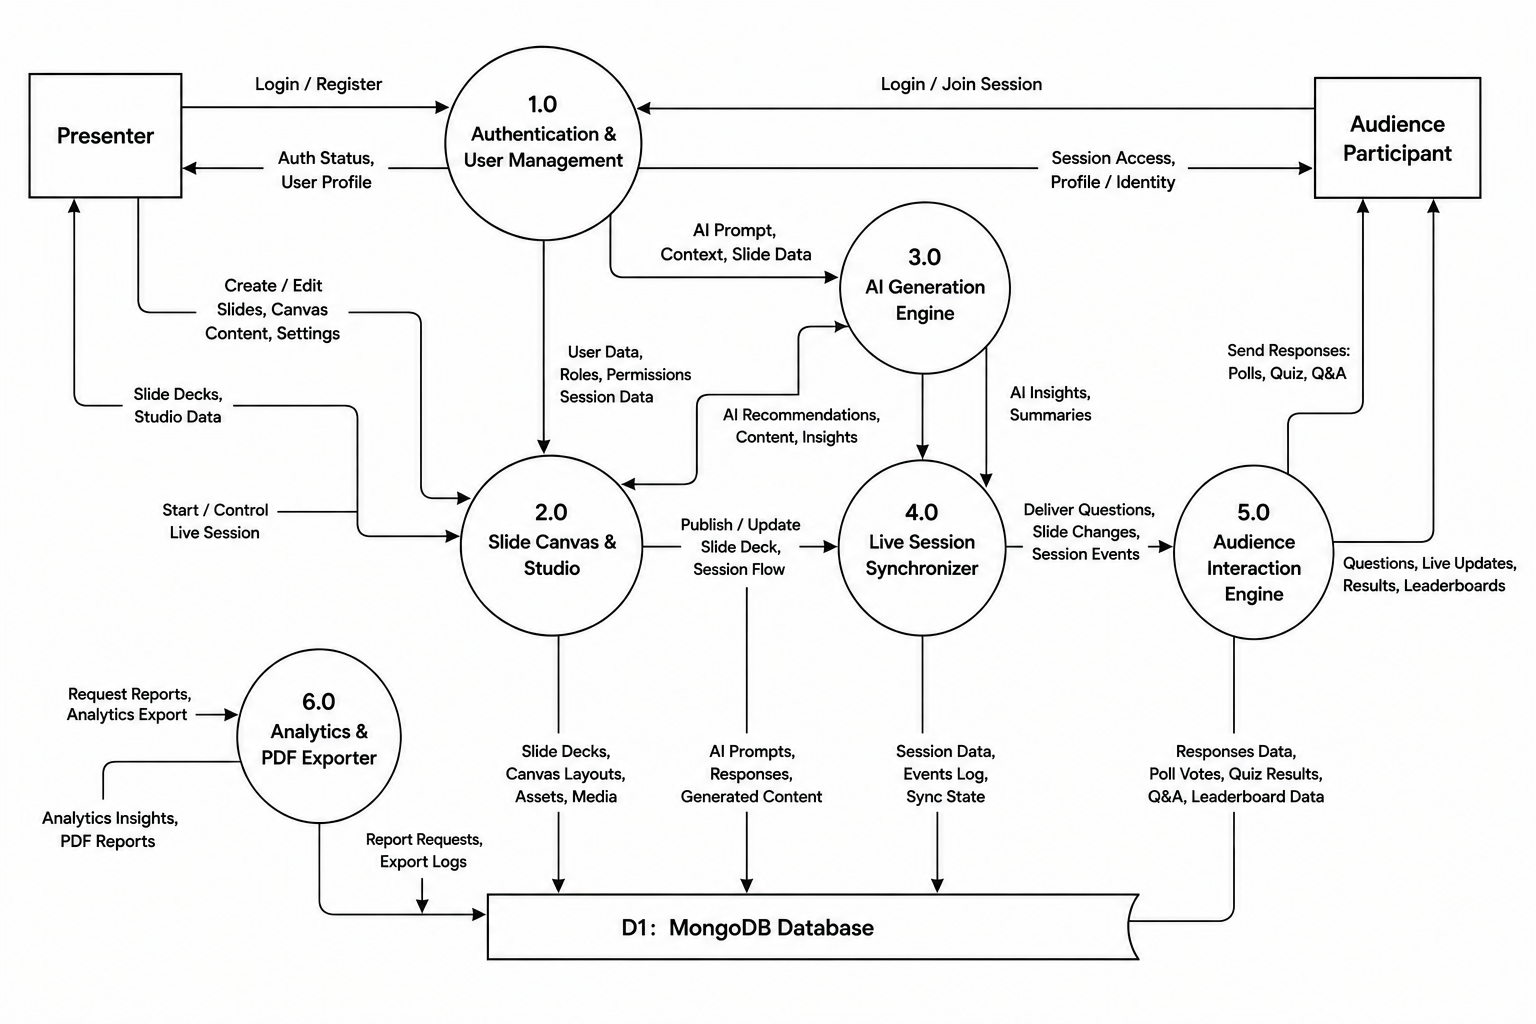
\includegraphics[width=0.9\textwidth]{figures/DFD_Level_1.png}
    \caption{Data Flow Diagram: Level 1}
    \label{fig:dfd1}
\end{figure}

\section{UML Modeling}

\subsection{Use Case Diagram}
Figure~\ref{fig:usecase} illustrates the core functional actions available to Presenters and Audience Participants.

\begin{figure}[H]
    \centering
    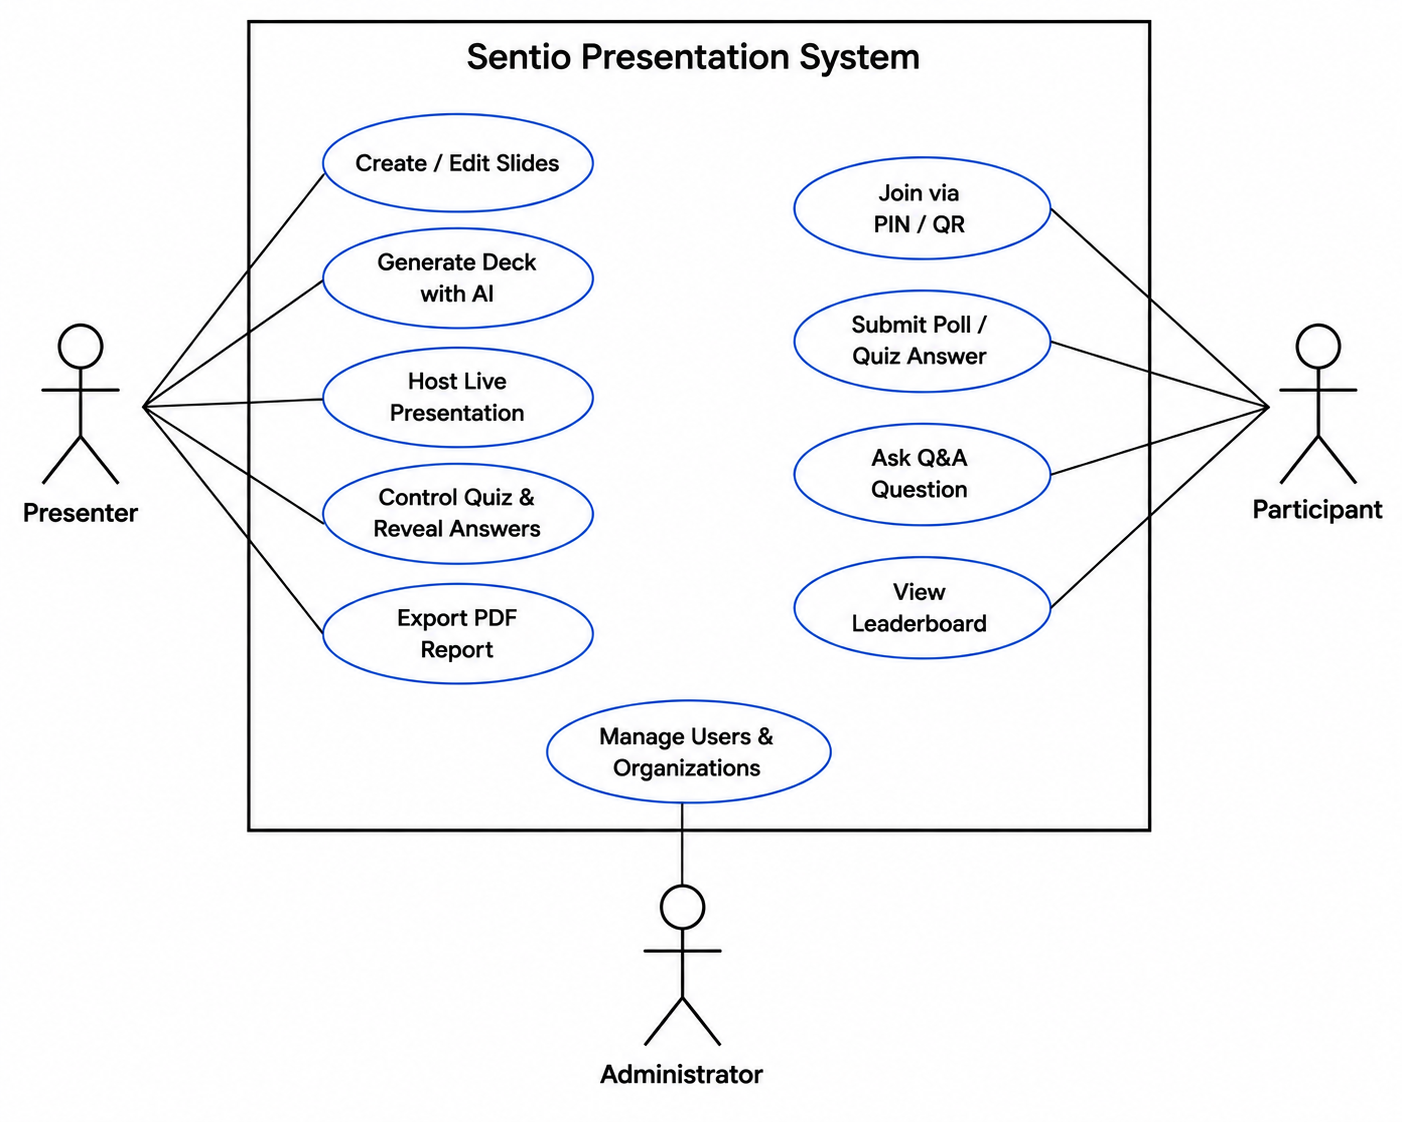
\includegraphics[width=0.85\textwidth]{figures/UML_UseCase.png}
    \caption{UML Use Case Diagram}
    \label{fig:usecase}
\end{figure}

\subsection{Sequence Diagram: Live Interaction}
Figure~\ref{fig:seqdiag} shows the step-by-step sequence of messages exchanged between the presenter, the server, and the audience during a live quiz question.

\begin{figure}[H]
    \centering
    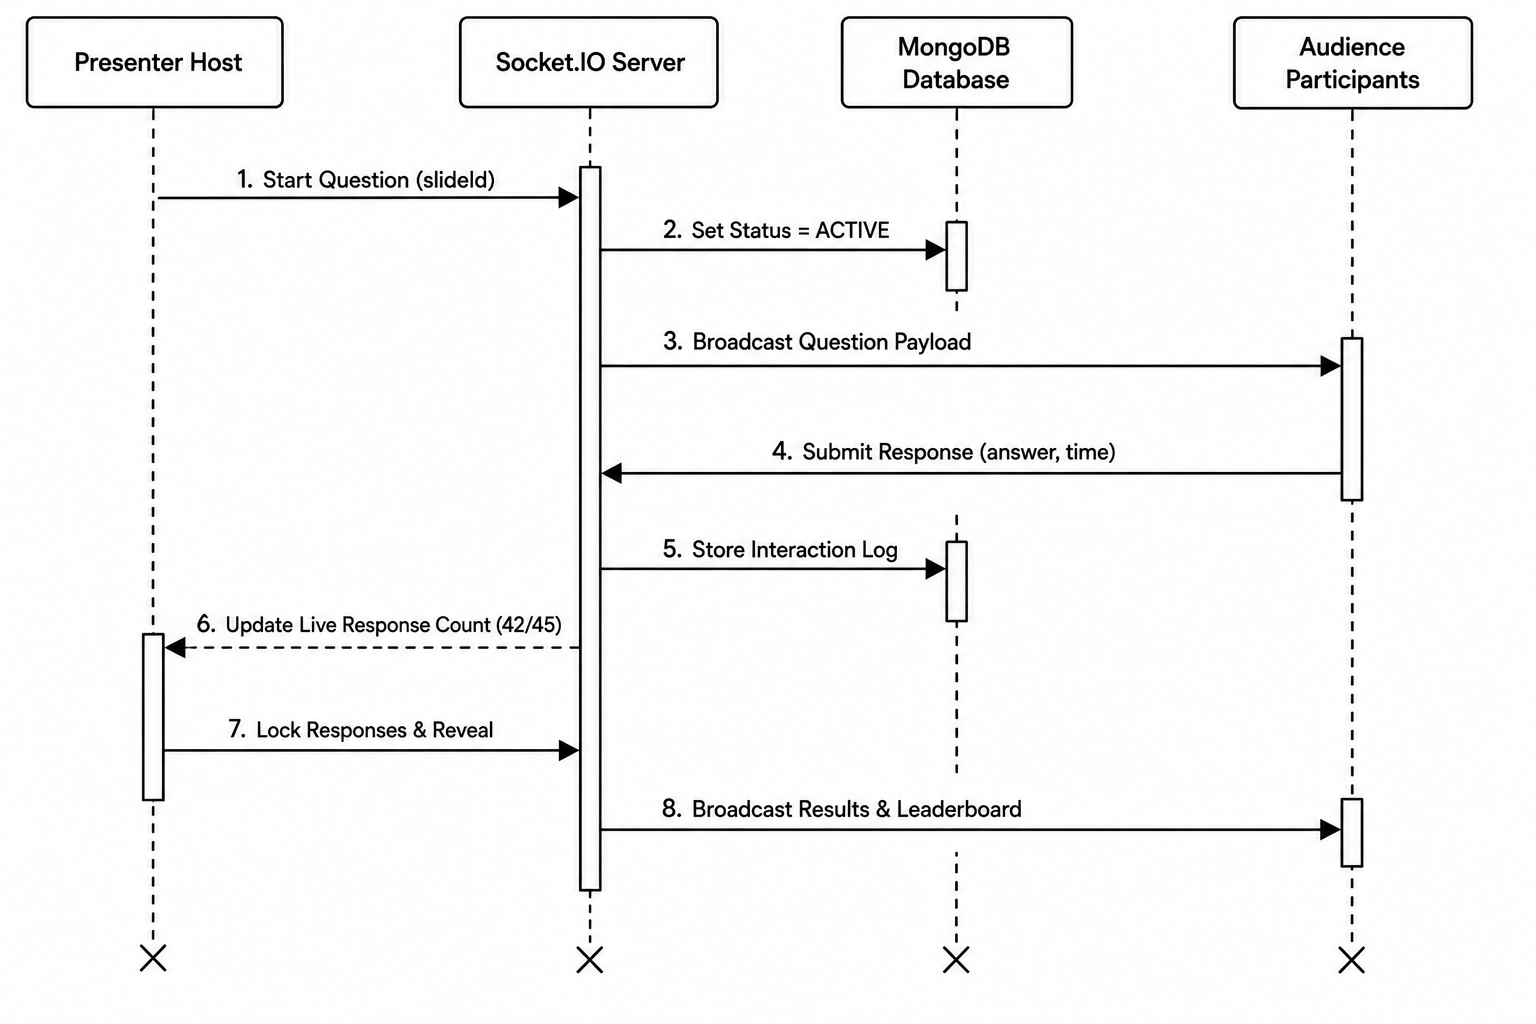
\includegraphics[width=0.85\textwidth]{figures/SequenceDiagram.png}
    \caption{Sequence Diagram for Live Question Flow}
    \label{fig:seqdiag}
\end{figure}

\section{Database Design}

Sentio uses MongoDB to store JSON-based presentation data. The primary collections are described below.

\begin{table}[H]
\centering
\caption{Users Collection (\texttt{users})}
\label{tab:userschema}
\begin{adjustbox}{max width=\textwidth}
\begin{tabular}{llcl}
\toprule
\textbf{Field} & \textbf{Type} & \textbf{Required} & \textbf{Description} \\
\midrule
\texttt{\_id} & ObjectId & Yes & Unique ID for the user \\
\texttt{name} & String & Yes & User's full name \\
\texttt{email} & String & Yes & Unique email address \\
\texttt{passwordHash} & String & Yes & Encrypted password \\
\texttt{role} & String & Yes & Role (\texttt{admin}, \texttt{presenter}, \texttt{participant}) \\
\texttt{createdAt} & Date & Yes & Account creation timestamp \\
\bottomrule
\end{tabular}
\end{adjustbox}
\end{table}

\begin{table}[H]
\centering
\caption{Presentations Collection (\texttt{presentations})}
\label{tab:presschema}
\begin{adjustbox}{max width=\textwidth}
\begin{tabular}{llcl}
\toprule
\textbf{Field} & \textbf{Type} & \textbf{Required} & \textbf{Description} \\
\midrule
\texttt{\_id} & ObjectId & Yes & Unique presentation ID \\
\texttt{title} & String & Yes & Title of the presentation \\
\texttt{creatorId} & ObjectId & Yes & Reference to user \\
\texttt{slidesCount} & Number & Yes & Number of slides in the deck \\
\texttt{createdAt} & Date & Yes & Creation timestamp \\
\bottomrule
\end{tabular}
\end{adjustbox}
\end{table}

\begin{table}[H]
\centering
\caption{Slide Elements Object Structure}
\label{tab:elemschema}
\begin{adjustbox}{max width=\textwidth}
\begin{tabular}{llcl}
\toprule
\textbf{Field} & \textbf{Type} & \textbf{Required} & \textbf{Description} \\
\midrule
\texttt{id} & String & Yes & Unique element ID \\
\texttt{type} & String & Yes & Element type (\texttt{text}, \texttt{image}, \texttt{quiz}, \texttt{poll}) \\
\texttt{x, y} & Number & Yes & Position on 16:9 canvas \\
\texttt{width, height} & Number & Yes & Size on canvas \\
\texttt{properties} & Object & No & Color, font size, and text values \\
\bottomrule
\end{tabular}
\end{adjustbox}
\end{table}
\chapter{Implementation and Results}

\section{Introduction}

The implementation phase translates the system design into working software. This chapter describes how the frontend, backend, real-time WebSocket communication, and AI features were built, tested, and evaluated across different screen sizes.

\section{Frontend Implementation}

The frontend is developed using \textbf{Next.js 15} with \textbf{React 19} and \textbf{TypeScript}. The user interface is broken down into clean, modular components:

\begin{itemize}
    \item \textbf{Slide Canvas (`SlideCanvas.tsx`):} A reusable component that detects the parent container's dimensions and applies a CSS scale transform to keep the slide in an exact 16:9 aspect ratio without shifting internal elements.
    \item \textbf{Slide Editor (`SlideEditor.tsx`):} The primary visual workspace where presenters can select, position, and edit slide elements.
    \item \textbf{Slide Navigator (`SlideNavigator.tsx`):} The left sidebar displaying slide thumbnails, allowing presenters to add, reorder, duplicate, and delete slides.
    \item \textbf{Interaction Components:} Specialized interactive components for multiple-choice Polls, timed Quizzes, Word Clouds, and Q\&A panels.
    \item \textbf{Auto-Save Hook (`useAutoSave.ts`):} A custom React hook that automatically saves slide edits after a brief 1.5-second pause in typing, preventing unnecessary API calls while ensuring work is never lost.
\end{itemize}

\section{Backend Implementation}

The backend API is built using \textbf{Node.js} and \textbf{Express.js} in `apps/backend/src`.

\subsection{Real-Time WebSocket Engine}
Real-time communication is managed using \textbf{Socket.IO v4}:
\begin{itemize}
    \item When a presenter starts a live session, the server generates a unique 6-character room PIN.
    \item When audience members join, their mobile browsers connect directly to this room.
    \item When the presenter advances a slide or launches a poll, the server broadcasts the update to all connected participant devices immediately.
    \item As audience members submit their answers, the server tallies the votes in memory and sends the updated live percentage distributions back to the presenter and projector screens in real time.
\end{itemize}

\subsection{AI Slide Generation}
The platform connects to the \textbf{Groq Cloud API} using the \textbf{LLaMA 3.3 70B} model. Presenters can enter a topic (such as ``Introduction to Cloud Computing'') and specify the number of slides desired. The AI generates a structured presentation deck complete with titles, bullet summaries, and relevant quiz questions in under two seconds.

\subsection{PDF Session Reports}
At the conclusion of a presentation, the backend uses \textbf{PDFKit} to generate a downloadable PDF report summarizing audience attendance, question-by-question response distributions, and participant scores.

\section{Testing and Evaluation}

The system was evaluated through automated test scripts as well as manual testing across different devices and screen resolutions.

\subsection{Automated Testing}
Unit and integration tests were written using Jest to test critical business logic:

\begin{table}[H]
\centering
\caption{Automated Test Results}
\label{tab:testresults}
\begin{adjustbox}{max width=\textwidth}
\begin{tabular}{lccc}
\toprule
\textbf{Test Category} & \textbf{Tests Executed} & \textbf{Passed} & \textbf{Status} \\
\midrule
User Authentication \& JWT & 14 & 14 & Passed \\
Presentation CRUD Operations & 18 & 18 & Passed \\
Canvas Scaling \& Element Models & 12 & 12 & Passed \\
Socket.IO Event Handlers & 16 & 16 & Passed \\
AI Response Formatter & 8 & 8 & Passed \\
Security \& Rate Limiting & 10 & 10 & Passed \\
\midrule
\textbf{Total} & \textbf{78} & \textbf{78} & \textbf{100\% Pass Rate} \\
\bottomrule
\end{tabular}
\end{adjustbox}
\end{table}

\subsection{Performance Benchmarks}
Measurements were taken during live sessions to ensure low-latency performance:

\begin{table}[H]
\centering
\caption{Performance Benchmarks}
\label{tab:perfresults}
\begin{adjustbox}{max width=\textwidth}
\begin{tabular}{lcc}
\toprule
\textbf{Metric} & \textbf{Expected Goal} & \textbf{Observed Result} \\
\midrule
Slide Broadcast Delay & $< 100\text{ ms}$ & $\mathbf{34\text{ ms}}$ \\
Participant Answer Ingestion & $< 50\text{ ms}$ & $\mathbf{22\text{ ms}}$ \\
AI 5-Slide Deck Generation & $< 3\text{ seconds}$ & $\mathbf{1.4\text{ seconds}}$ \\
PDF Report Creation Time & $< 2\text{ seconds}$ & $\mathbf{0.6\text{ seconds}}$ \\
\bottomrule
\end{tabular}
\end{adjustbox}
\end{table}

\section{System Views}

Figure~\ref{fig:screenslayout} illustrates the multi-screen coordination between the presenter, the audience, and the projector.

\begin{figure}[H]
    \centering
    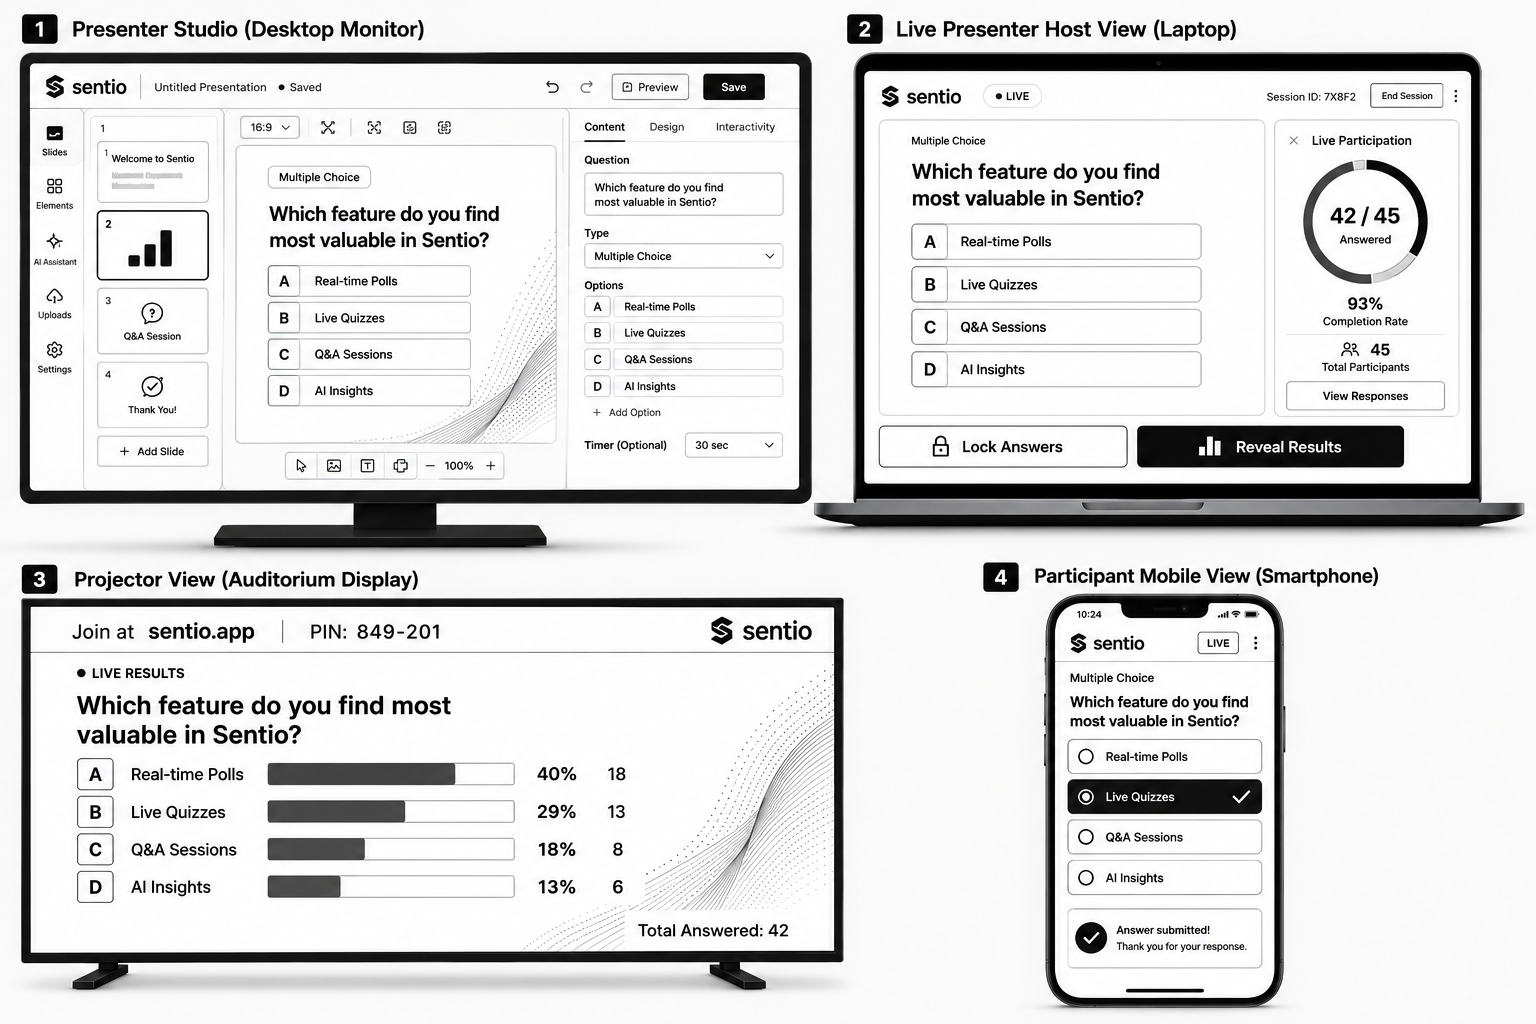
\includegraphics[width=0.9\textwidth]{figures/SynchronizedViewsAcrossDifferentDevices.png}
    \caption{Synchronized Views Across Different Devices}
    \label{fig:screenslayout}
\end{figure}
\chapter{Conclusion and Future Scope}

\section{Conclusion}

The \textbf{Sentio} project was developed to transform traditional, one-sided presentations into interactive, two-way learning and engagement experiences. By combining a flexible 16:9 slide canvas, real-time WebSockets, and fast AI generation, Sentio eliminates the friction of switching between multiple disconnected presentation and polling tools.

The key outcomes of the project include:
\begin{enumerate}
    \item \textbf{16:9 Responsive Canvas:} A reliable slide layout that maintains exact visual placement across all screen sizes without reflowing content.
    \item \textbf{Integrated Interaction Suite:} Native support for live quizzes, polls, word clouds, rating scales, Q\&A, and competitive leaderboards on slides.
    \item \textbf{Fast Real-Time Updates:} A Socket.IO WebSocket backend that updates audience responses and slide changes in under 40 milliseconds.
    \item \textbf{AI-Assisted Slide Creation:} Integration with Groq AI (LLaMA 3.3) for generating structured slide decks and quizzes in under two seconds.
    \item \textbf{Automated Reporting:} Generation of downloadable session summary reports in PDF format.
\end{enumerate}

\section{Limitations}

The current version of the system has the following practical limitations:
\begin{itemize}
    \item \textbf{Internet Connectivity Dependency:} Real-time polling and response synchronization require an active internet connection on presenter and audience devices.
    \item \textbf{Single Primary Presenter Control:} While multi-tenant organizations are supported, simultaneous real-time co-presenter dual-control of an active session is currently limited.
\end{itemize}

\section{Future Scope}

Future enhancements planned for the platform include:
\begin{enumerate}
    \item \textbf{Real-Time Voice Transcription:} Using speech recognition to transcribe the speaker's voice during talks and automatically highlight key terms on slides.
    \item \textbf{Adaptive Presentation Paths:} Enabling AI to suggest alternative review slides dynamically based on how well the audience answers a quiz question.
    \item \textbf{Native Mobile Companion App:} Creating dedicated mobile apps for iOS and Android with haptic feedback and remote slide clicker controls.
    \item \textbf{LMS Integration:} Connecting quiz scores and attendance directly to Learning Management Systems such as Moodle and Google Classroom.
\end{enumerate}


% =================================================
% REFERENCES
% =================================================

\begin{thebibliography}{99}

\bibitem{nextjs}
Vercel, ``Next.js 15 Documentation \& App Router Architecture,'' \url{https://nextjs.org/docs}, 2025.

\bibitem{react19}
Meta Open Source, ``React 19 Documentation: Server Components \& Actions,'' \url{https://react.dev}, 2025.

\bibitem{socketio}
Socket.IO Foundation, ``Socket.IO v4: Realtime Bidirectional Event-Based Communication,'' \url{https://socket.io/docs/v4/}, 2024.

\bibitem{express}
OpenJS Foundation, ``Express.js: Fast, Unopinionated, Minimalist Web Framework for Node.js,'' \url{https://expressjs.com}, 2024.

\bibitem{mongodb}
MongoDB Inc., ``MongoDB Manual: Document-Based Distributed Database Architecture,'' \url{https://www.mongodb.com/docs/}, 2025.

\bibitem{groq}
Groq Inc., ``LPU Inference Engine \& Ultra-Low Latency LLM Serving API (LLaMA 3.3 70B),'' \url{https://groq.com}, 2025.

\bibitem{tailwind}
Tailwind Labs, ``Tailwind CSS v4: Utility-First CSS Framework Architecture,'' \url{https://tailwindcss.com/docs}, 2025.

\bibitem{framer}
Framer B.V., ``Framer Motion: Production-Ready Motion Library for React,'' \url{https://www.framer.com/motion/}, 2024.

\end{thebibliography}

\end{document}